% Pretraining learning curves — masked-modelling loss vs step, one line per dataset backbone.
\begin{figure}[t]
\centering
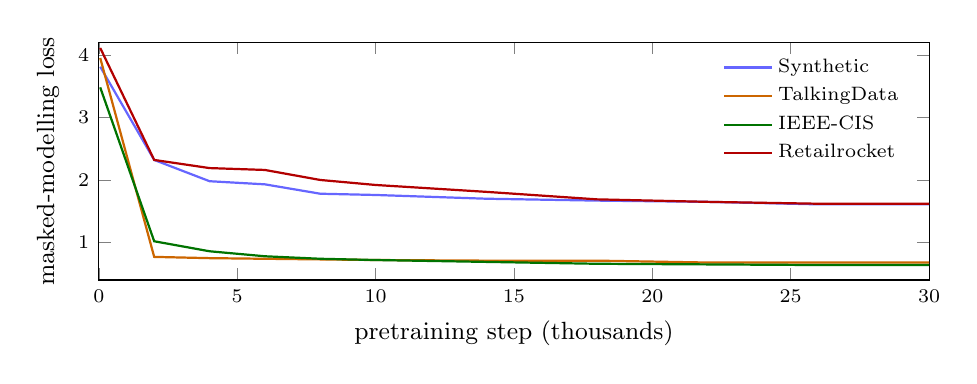
\begin{tikzpicture}
\begin{axis}[width=\linewidth, height=4.6cm,
  xlabel={pretraining step (thousands)}, ylabel={masked-modelling loss},
  xlabel near ticks, ylabel near ticks, xmin=0, xmax=30, ymin=0.4, ymax=4.2,
  legend style={font=\scriptsize, at={(0.98,0.98)}, anchor=north east, draw=none, fill=none},
  legend cell align=left, tick label style={font=\scriptsize}, label style={font=\small}]
\addplot[blue!60, thick] coordinates {(0.05,3.81)(2,2.32)(4,1.98)(6,1.93)(8,1.78)(10,1.76)(14,1.70)(18,1.67)(22,1.65)(26,1.61)(30,1.61)};
\addlegendentry{Synthetic}
\addplot[orange!80!black, thick] coordinates {(0.05,3.95)(2,0.77)(4,0.75)(6,0.74)(10,0.72)(14,0.71)(18,0.71)(22,0.68)(26,0.68)(30,0.68)};
\addlegendentry{TalkingData}
\addplot[green!45!black, thick] coordinates {(0.05,3.48)(2,1.02)(4,0.86)(6,0.78)(8,0.74)(10,0.72)(14,0.69)(18,0.66)(22,0.65)(26,0.64)(30,0.64)};
\addlegendentry{IEEE-CIS}
\addplot[red!70!black, thick] coordinates {(0.05,4.11)(2,2.32)(4,2.19)(6,2.16)(8,2.00)(10,1.92)(14,1.81)(18,1.69)(22,1.65)(26,1.62)(30,1.62)};
\addlegendentry{Retailrocket}
\end{axis}
\end{tikzpicture}
\caption{Masked-modelling pretraining loss for each dataset's backbone. Every curve plateaus well
before \num{30000} steps, so each FFM is converged before any adaptation.}
\label{fig:loss}
\end{figure}
